\begin{flushright}
    فرض کنید می‌خواهیم یک فایل را در حافظه ذخیره‌سازی کنیم.
    اگر به دید انتزاعی به حافظه و فایل نگاه کنیم.
    نحوه قرار گیری فایل در حافظه به صورت زیر خواهد بود.

    \begin{figure}[H]
        \centering
        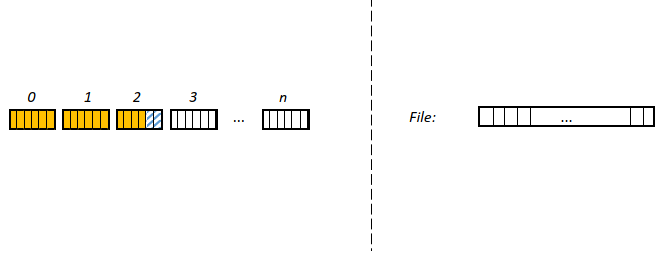
\includegraphics[width=0.7\textwidth]{source/file-in-memory-model-1}
        \caption{نحوه ذخیره‌سازی فایل در حافظه}
        \label{fig:file-in-memory-model-1}
    \end{figure}

    در این شیوه ذخیره‌سازی فایل در حافظه به درستی ذخیره می‌شود اما اگر بخواهیم همان فایل را بخوانیم نیاز داریم تا اندازه فایل را بدانیم.
    برای رفع این مشکل می‌توانیم تعدادی از بلوک‌های اولیه را به اطلاعاتی در مورد فایل(مانند اندازه فایل) اختصاص دهیم.

    \begin{figure}[H]
        \centering
        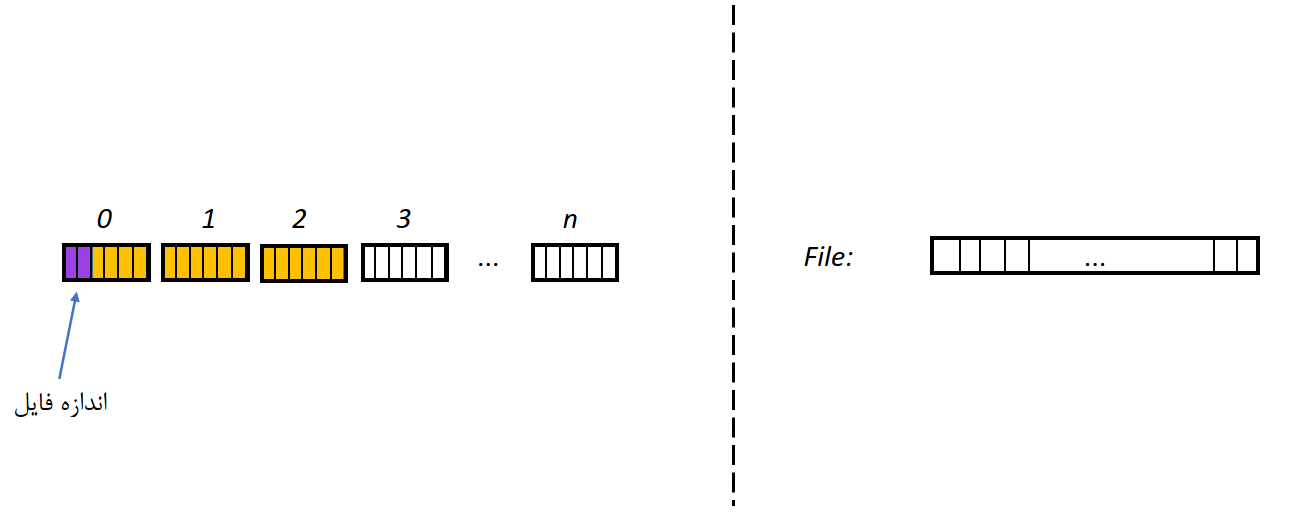
\includegraphics[width=0.7\textwidth]{source/file-in-memory-model-2}
        \caption{نحوه ذخیره‌سازی فایل در حافظه به همراه اطلاعات فایل}
        \label{fig:file-in-memory-model-2}
    \end{figure}

    حال فرض کنید قسمتی از این فایل را حذف کنیم.
    در این صورت چه تغغیراتی در شیوه ذخیره‌سازی لازم خواهد بود.

    \begin{figure}[H]
        \minipage{0.5\textwidth}
        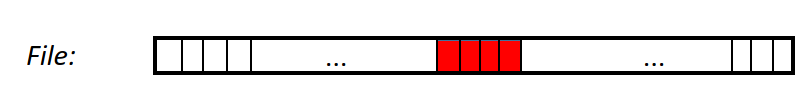
\includegraphics[width=\linewidth]{source/file-deleted-parts}
        \caption{فایلی که قسمت‌هایی از آن پاک شده است.}\label{fig:file-deleted-parts}
        \endminipage\hfill
        \minipage{0.5\textwidth}
        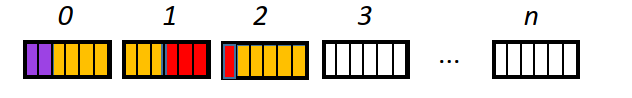
\includegraphics[width=\linewidth]{source/file-in-memory-model-3}
        \caption{فایل تغییر یافته در حافظه}\label{fig:file-in-memory-model-3}
        \endminipage\hfill
    \end{figure}

    یک روش برای حل این مشکل، شیفت دادن متوالی بلوک‌ها به سمت چپ است.
    تا اطلاعات فایل دوباره به صورت بلوک‌های متوالی ذخیره شود.

    \begin{figure}[H]
        \centering
        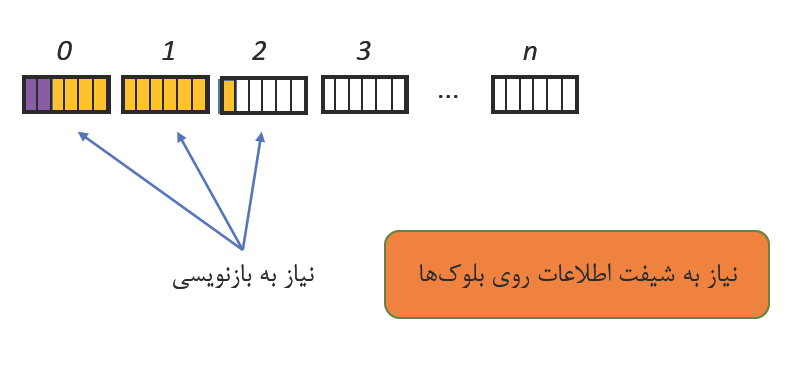
\includegraphics[width=0.7\textwidth]{source/shift-file}
        \caption{بازنویسی فایل در حافظه}
        \label{fig:shift-file}
    \end{figure}

    هرچند این روش کارایی سیستم را در اثر ایجاد تغییرات در فایل بسیار پایین می‌آورد.

    روش دیگری که می‌تواینم استفاده کنیم تا کارایی را افزایش دهیم، استفاده از
    لیست پیوندی
    \footnote{list linked}
    می‌باشد.

    \begin{figure}[H]
        \centering
        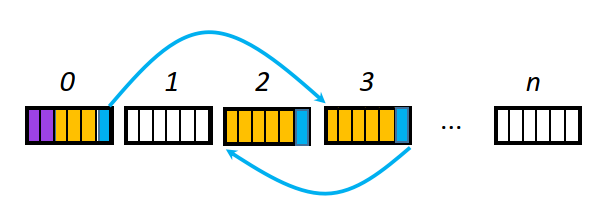
\includegraphics[width=0.7\textwidth]{source/file-in-memory-model-4}
        \caption{فایل در حافظه با استفاده از لیست پیوندی}
        \label{fig:file-in-memory-model-4}
    \end{figure}

    دقت شود که برای آنکه بتوانیم از لیست پیوندی استفاده کنیم، نیاز داریم بدانیم چه تعداد از فضای یک بلوک اشغال شده است.
    این اطلاعات را می‌توان در خانه ابتدایی بلوک ذخیره کنیم.

    \begin{figure}[H]
        \centering
        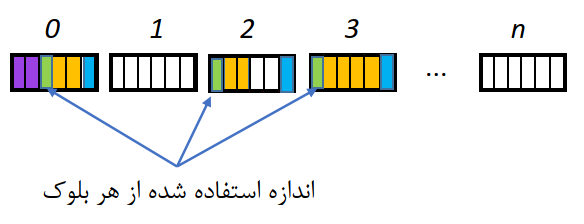
\includegraphics[width=0.7\textwidth]{source/file-in-memory-model-5}
        \caption{ذخیره‌سازی فایل در حافظه به همراه اندازه استفاده شده از هر بلوک}
        \label{fig:file-in-memory-model-5}
    \end{figure}

    می‌توانیم انتزاعی فراتر داشته باشیم تا از جزئیات چگونگی ذخیره‌سازی دوری کنیم در ادامه بحث با این انتزاع آشنا خواهیم شد.
\end{flushright}